\documentclass[10pt,a4j,twocolumn]{jsarticle}

\usepackage[dvipdfmx]{graphicx}
\usepackage{wrapfig}

\setlength{\textheight}{275mm}
\headheight 5mm
\topmargin -30mm
\textwidth 185mm
\oddsidemargin -15mm
\evensidemargin -15mm
\pagestyle{empty}
\begin{document}
\title{RubyでMapleを動かすためのインターフェースの開発}
\author{情報科学科 西谷研究室 3528 村瀬愛理}
\date{}
\maketitle
\section{研究目的}
Rubyでは数値計算のライブラリ開発が遅れており,Ruby上では高等な関数(素数を求めたり,最小公倍数を求めるなど)を使った数式処理を行うのが難しい.また,Ruby以外の数式処理ソフトウェアを別に立ち上げて別々で作業したり慣れない別の言語を勉強し直したりするよりも,Rubyのみでプログラミングする方が開発速度の格段の向上が期待できる.そこで本研究では,MapleをRuby上で呼び出し,Mapleに高等な関数や桁数の大きな数値を用いた計算をさせて,その結果をRubyが取得するインターフェースライブラリの開発を目的とする.

\section{手法}
\subsection{Mapleとは}
Mapleは,1980年にカナダ・ウォータールー大学で生まれた数式処理技術をコアテクノロジーとして持つ科学・技術・工学・数学(STEM : Science, Technology, Engineering and Mathematics)に関する統合的計算環境である[1].特徴として,たくさんの数学関数が用意されていること,大きな桁数の計算が可能であること,グラフの描画が簡単であり,かつ3次元のグラフの描画にも対応していることなどが挙げられる.数式を入力するだけで簡単に解を得ることができることから,多くの場で用いられている.

\subsection{Mapleとの通信手法}
Mapleは一般的に,グラフや数式の綺麗な出力や,数式の入力を初心者が直感的におこなえるようにJavaで作られたGUIを使って実行する.それとは別にcommand lineで実行される計算エンジン部が用意されている.そこで,開発するRubyライブラリでは,このエンジンに直接働きかけて操作する.Rubyで外部コマンドを実行するgem libraryのsystemuを使って,出力を得るようにしている.Ruby codeで要求コードを受け取った場合,そのコードをtmp.mwに書き込む.それをMapleで実行し,結果をテキストファイルで受けとることで出力を得る.

\subsection{Maple関数の類型化,出力の切り替え}
今回,数多く存在するMapleの数学関数の中から整数論と行列に関するものを選抜し実装した後,入出力に関して類型化し,それぞれの出力に応じてwrapperを作った.

\section{基本動作}
入力された値の次の素数を出力するnextprimeを用いて説明する.
\begin{wrapfigure}{r}{4cm}\begin{center}
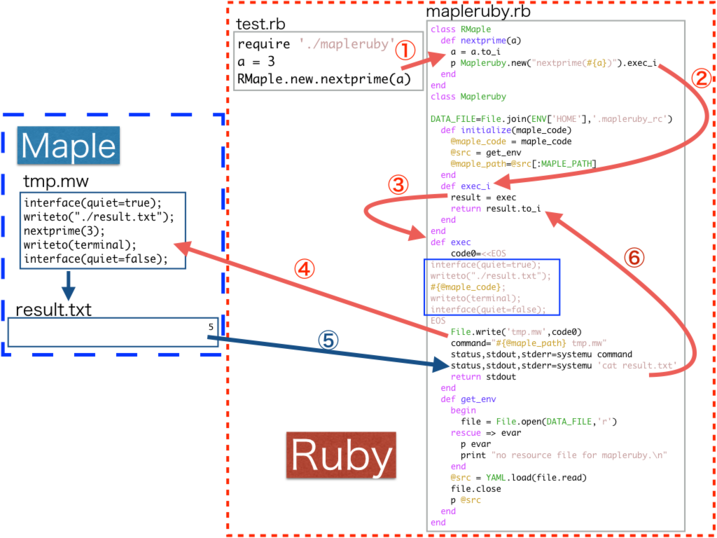
\includegraphics[width=6cm, bb=0 0  937 753]{./mapleruby_eringi.003.png}
\caption{(figure:one)maplerubyの基本動作.}
\label{default}\end{center}\end{wrapfigure}

\begin{enumerate}
\item maplerubyをrequireした上で使いたい関数を使う.RMaple.new.hogehogeのhogehogeに使いたい関数名を入れる.今回はnextprimeで説明を進める.
\item RMapleクラス内のnextprime関数が呼び出され,aに3が入る.この時nextprimeは入力された値がint型になるように関数内でto\_iしてある.その後,Maplerubyクラスのexec\_i関数へ"nextprime(3)"が出力される.この出力された文字列がそのままMapleでの計算に使われる.
\item 出力された文字列をさらにexec関数へ出力する.
\item 青四角内の内容をMapleへと出力する.この時\verb|#{@maple_code};|となっている部分に先ほどの"nextprime(3)"が入る.青四角の内容がMapleに出力され実行されることで得られた答えがresult.txtに出力されるようになっている.
\item result.txtに出力された内容をRuby側で受け取り,exec\_iに再び返す.
\item 返された値をto\_iすることでint型に直して解を出力する.
\end{enumerate}
\section{本研究による成果}
本研究で得られた成果をまとめると以下の通りである.

\begin{itemize}
\item RSA暗号化における計算が,Ruby単体で行うよりも約100倍の数まで扱えるようになった.
\item 3行3列の行列について逆行列や固有値,固有ベクトルを求めることができた.
\end{itemize}
従来MapleとRubyを行き来しなければならなかった計算でも,maplerubyを用いることでRuby上のみで完結させられるようになった.またRuby上のみで計算ができるようになったため,RubyライブラリにあるTest::Unitと並行して使用すれば,求めたい解が分かっている際に自分が書いたプログラムで正しく解が導けるのかテストすることも可能になった.

\section{総括}
Rubyだけで桁数の大きい計算や複雑な数学関数を必要とする計算を完結させられることが可能になった.今後は現状Maplerubyクラスに直接送っている累乗,四則混合などの基本的な計算や,等式の解を出力する関数evalなど新たな関数の追加,さらにMapleの特徴である綺麗なグラフ描画ができることを生かし,グラフの出力を可能にするなどの課題が挙げられる.

\section{参考文献}
[1]「Maple(メイプル) とは」, サイバネット, \verb|http://www.cybernet.co.jp/maple/product/maple/about.html,| 2017/02/01アクセス.
\end{document}
